\newpage
\section{Bridge Pattern}

Bridge is used when we need to decouple an abstraction from its implementation so that the two can vary independently. This type of design pattern comes under structural pattern as this pattern decouples implementation class and abstract class by providing a bridge structure between them.

This pattern involves an interface which acts as a bridge which makes the functionality of concrete classes independent from interface implementer classes. Both types of classes can be altered structurally without affecting each other.

We are demonstrating use of Bridge pattern via following example in which a circle can be drawn in different colors using same abstract class method but different bridge implementer classes. 

\subsection{Implementation}

We have a DrawAPI interface which is acting as a bridge implementer and concrete classes RedCircle, GreenCircle implementing the DrawAPI interface. Shape is an abstract class and will use object of DrawAPI. BridgePatternDemo, our demo class will use Shape class to draw different colored circle.

\subsection{Class Diagram}

\begin{figure}[h]
\centering
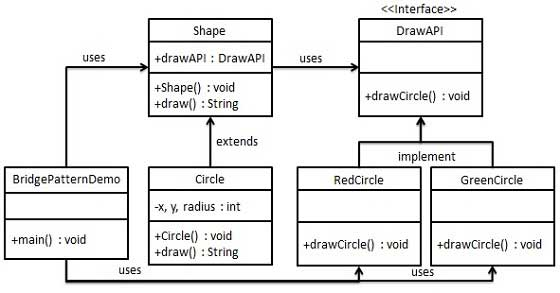
\includegraphics[scale=0.7]{bridge}
\caption{Class Diagram of Bridge Pattern}
\end{figure}

\newpage
\subsection{Source Code (Java)}

\subsubsection{DrawAPI Interface}

\begin{minted}{java}
public interface DrawAPI {
   public void drawCircle(int radius, int x, int y);
}
\end{minted}

\subsubsection{RedCircle Class}

\begin{minted}{java}
public class RedCircle implements DrawAPI {
   @Override
   public void drawCircle(int radius, int x, int y) {
      System.out.println(
		"Drawing Circle[ color: red, radius: " + radius + ", x: " + x + ", " + y + "]"
	);
   }
}
\end{minted}

\subsubsection{GreenCircle Class}

\begin{minted}{java}
public class GreenCircle implements DrawAPI {
   @Override
   public void drawCircle(int radius, int x, int y) {
      System.out.println(
		"Drawing Circle[ color: green, radius: " + radius + ", x: " + x + ", " + y + "]"
	);
   }
}
\end{minted}

\subsubsection{Shape abstract Class}

\begin{minted}{java}
public abstract class Shape {
   protected DrawAPI drawAPI;
   
   protected Shape(DrawAPI drawAPI){
      this.drawAPI = drawAPI;
   }
   public abstract void draw();	
}
\end{minted}

\subsubsection{Circle Class}

\begin{minted}{java}
public class Circle extends Shape {
   private int x, y, radius;

   public Circle(int x, int y, int radius, DrawAPI drawAPI) {
      super(drawAPI);
      this.x = x;  
      this.y = y;  
      this.radius = radius;
   }

   public void draw() {
      drawAPI.drawCircle(radius,x,y);
   }
}
\end{minted}

\subsubsection{Driver Class}

\begin{minted}{java}
public class BridgePatternDemo {
   public static void main(String[] args) {
      Shape redCircle = new Circle(100,100, 10, new RedCircle());
      Shape greenCircle = new Circle(100,100, 10, new GreenCircle());

      redCircle.draw();
      greenCircle.draw();
   }
}
\end{minted}

\subsection{Output}

\begin{minted}{text}
Drawing Circle[ color: red, radius: 10, x: 100, 100]
Drawing Circle[  color: green, radius: 10, x: 100, 100]
\end{minted}
